\documentclass{article}
\usepackage{amsmath, amssymb, graphicx}
\usepackage{caption}
\usepackage{float}
\title{Lissajous Figures: A Mathematical Perspective}
\author{EE24BTECH11048:NITHIN.K,\\EE24BTECH11021:ESHAN RAY}
\date{\today}

\begin{document}
\maketitle
\section{Function Generator}

\subsection{Definition}
A function generator is an electronic device that produces different types of waveforms over a range of frequencies.

\subsection{Types of Waveforms}
\begin{itemize}
    \item \textbf{Sine Wave} – Smooth periodic oscillations.
    \item \textbf{Square Wave} – Alternating high and low levels.
    \item \textbf{Triangular Wave} – Linear rise and fall.
    \item \textbf{Sawtooth Wave} – Gradual rise with a sudden drop.
    \item \textbf{Pulse Wave} – Short-duration high signals.
\end{itemize}

\subsection{Frequency Range}
Function generators typically operate in the range of a few mHz to several MHz, depending on the model.

\subsection{Duty Cycle Adjustment}
\begin{itemize}
    \item The duty cycle controls the proportion of the waveform's high time to its period.
    \item Useful for PWM (Pulse Width Modulation) applications.
\end{itemize}

\subsection{Amplitude and Offset Control}
\begin{itemize}
    \item The output amplitude can be adjusted.
    \item DC Offset allows shifting the waveform above or below zero volts.
\end{itemize}

\subsection{Modulation Capabilities}
Some function generators support AM (Amplitude Modulation), FM (Frequency Modulation), and PM (Phase Modulation).

\subsection{Sweep Function}
\begin{itemize}
    \item Allows gradual frequency change over a set range.
    \item Used for testing frequency response in circuits.
\end{itemize}

\subsection{Applications}
\begin{itemize}
    \item Testing amplifiers and filters.
    \item Signal processing experiments.
    \item Debugging and troubleshooting electronic circuits.
    \item Generating clock pulses for digital circuits.
\end{itemize}

\begin{figure}[H]
\centering
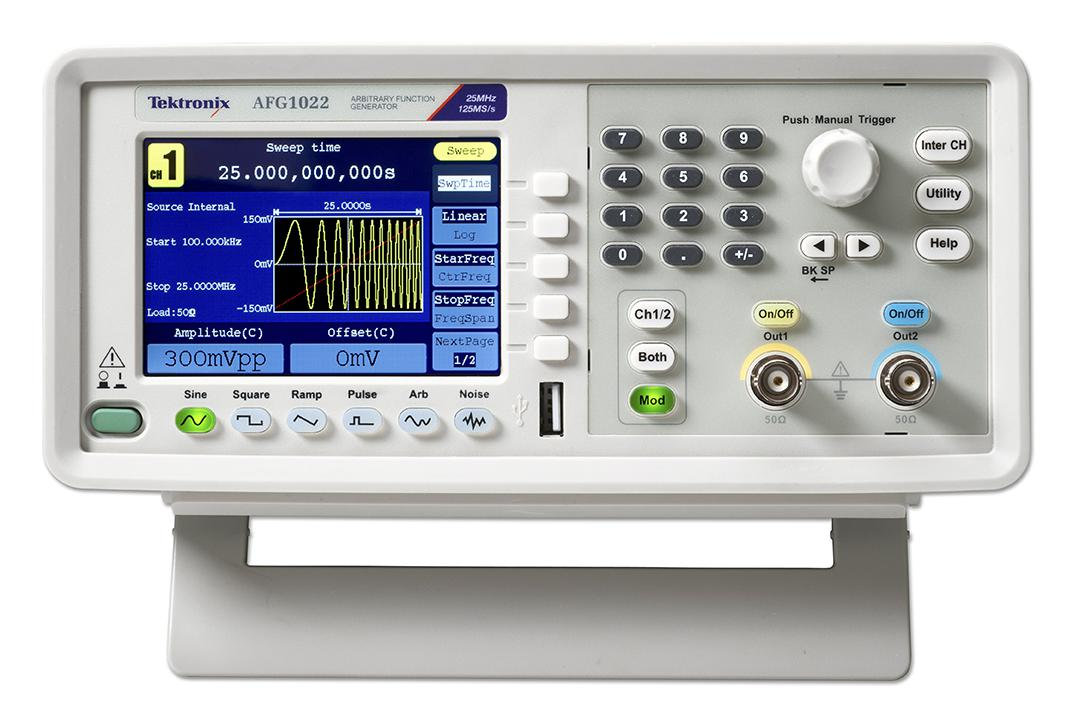
\includegraphics[width=0.5\textwidth]{figs/func_gen.png}
\caption{Function Generator}
\end{figure}

\begin{abstract}
Lissajous figures are complex and beautiful patterns formed by the parametric equations of two perpendicular harmonic oscillations. This report explores their mathematical representation, properties, and applications in various fields such as physics, engineering, and art.
\end{abstract}

\section{Introduction}
Lissajous figures, named after the French mathematician Jules Antoine Lissajous, are the graphs of parametric equations describing two harmonic motions in perpendicular directions. These figures are useful in analyzing the relationship between two oscillatory signals and are commonly seen in physics, engineering, and signal processing.

\section{Mathematical Representation}
The general parametric equations for Lissajous figures are:
\begin{equation}
x(t) = A \sin(\omega_x t + \delta)
\end{equation}
\begin{equation}
y(t) = B \sin(\omega_y t)
\end{equation}
where:
\begin{itemize}
\item $A$ and $B$ are the amplitudes of the oscillations,
\item $\omega_x$ and $\omega_y$ are the angular frequencies,
\item $\delta$ is the phase difference between the two oscillations,
\item $t$ is the time parameter.
\end{itemize}

\section{Properties of Lissajous Figures}
Lissajous figures exhibit various properties depending on the frequency ratio $\frac{\omega_x}{\omega_y}$ and the phase difference $\delta$:
\begin{itemize}
\item When the frequencies are in simple integer ratios (e.g., 1:1, 2:3), closed curves form.
\item If $\omega_x = \omega_y$ and $\delta = \frac{\pi}{2}$, the figure is a circle.

\begin{figure}[H]
\centering
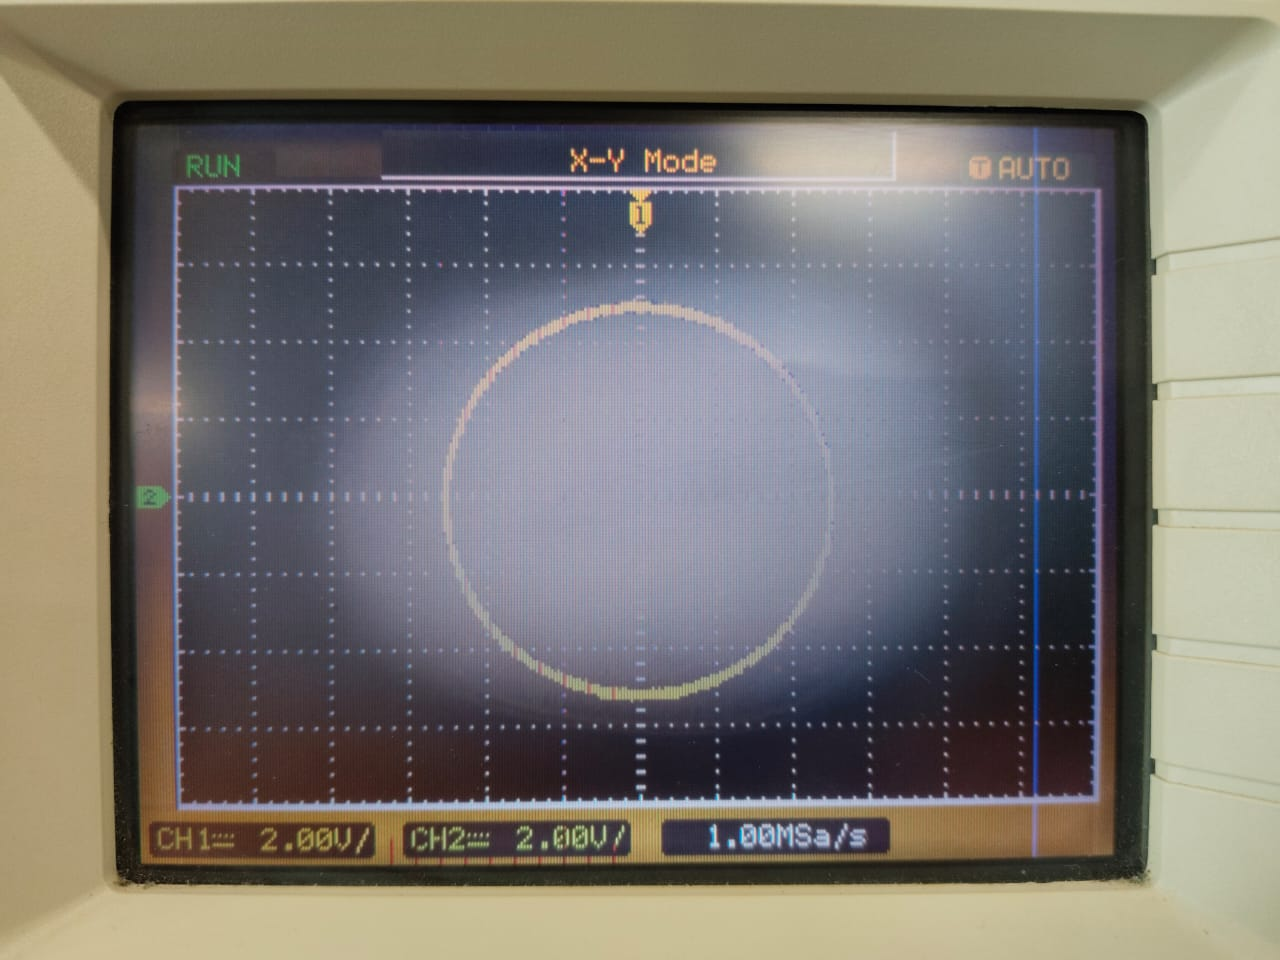
\includegraphics[width=0.5\textwidth]{figs/fig.png}
\end{figure}

\item More complex ratios and phase differences result in intricate patterns.
\item Their symmetry properties depend on the phase shift and amplitude ratios.
\end{itemize}

\section{Applications of Lissajous Figures}
Lissajous figures have applications in various domains, including:
\begin{itemize}
\item \textbf{Oscilloscope Applications:} Used to visualize the phase relationship between two signals.
\item \textbf{Vibration Analysis:} Employed to analyze harmonic motion in mechanical systems.
\item \textbf{Signal Processing:} Used to study frequency components of audio and electrical signals.
\item \textbf{Art and Design:} Generate aesthetically appealing patterns.
\end{itemize}

\section{Analysis of Given Specifications}
Below are various Lissajous figure specifications and their corresponding mathematical solutions.

\subsection{Case 1: $y = \sin(3\text{kHz})$, $x = \sin(5\text{kHz} + 90^\circ)$}

Given:
\[
x(t) = \sin(2\pi \cdot 5000 t + \frac{\pi}{2})
\]
\[
y(t) = \sin(2\pi \cdot 3000 t)
\]
\begin{align*}
x^2 + y^2 = \cos^2(2\pi \cdot 5000t) + \sin^2(2\pi \cdot 3000t)
\end{align*}
The frequencies are \( \omega_x = 2\pi \cdot 5000 \) and \( \omega_y = 2\pi \cdot 3000 \). The frequency ratio is:
\[
\frac{\omega_x}{\omega_y} = \frac{5000}{3000} = \frac{5}{3}
\]

Since the phase difference is \( 90^\circ = \frac{\pi}{2} \), the figure will be symmetric and display a characteristic pattern with a quarter-period phase shift between the axes.
\begin{figure}[H]
\centering
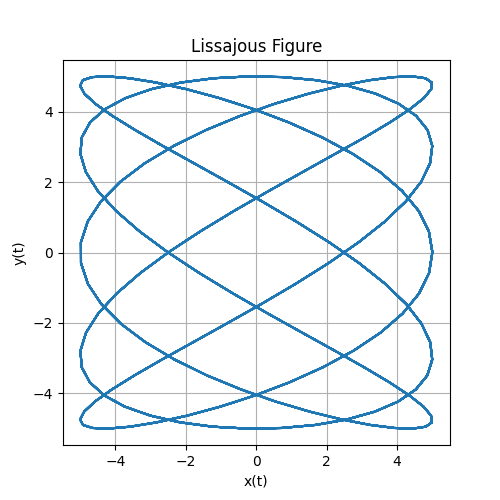
\includegraphics[width=0.5\textwidth]{figs/fig1.png}
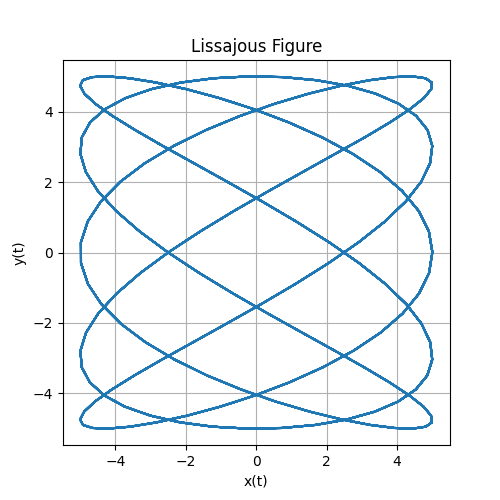
\includegraphics[width=0.5\textwidth]{figs/fig1_verify.png}
\end{figure}
\subsection{Case 2: $y = \sin(3\text{kHz})$, $x = \sin(4\text{kHz} + 45^\circ)$}

Given:
\[
x(t) = \sin(2\pi \cdot 4000 t + \frac{\pi}{4})
\]
\[
y(t) = \sin(2\pi \cdot 3000 t)
\]
\begin{align*}
x^2 + y^2 = \frac{1}{2} + \frac{1}{2} \sin\left( 4\pi \cdot 4000 t \right) + \sin^2\left( 2\pi \cdot 3000 t \right)
\end{align*}
The frequency ratio is:
\[
\frac{\omega_x}{\omega_y} = \frac{4000}{3000} = \frac{4}{3}
\]

The phase difference is \( 45^\circ = \frac{\pi}{4} \), which will result in a more complex Lissajous pattern. The graph will have intricate loops with slight skewing.
\begin{figure}[H]
\centering
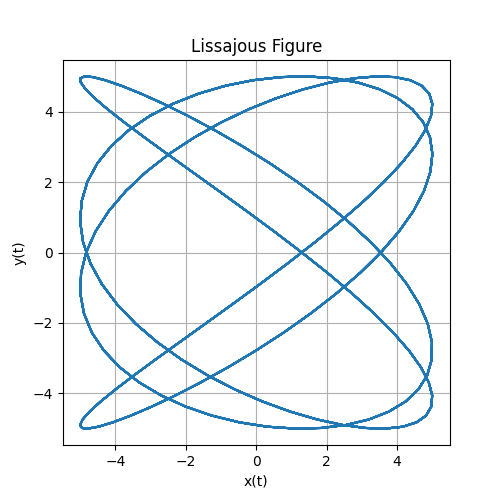
\includegraphics[width=0.5\textwidth]{figs/fig2.png}
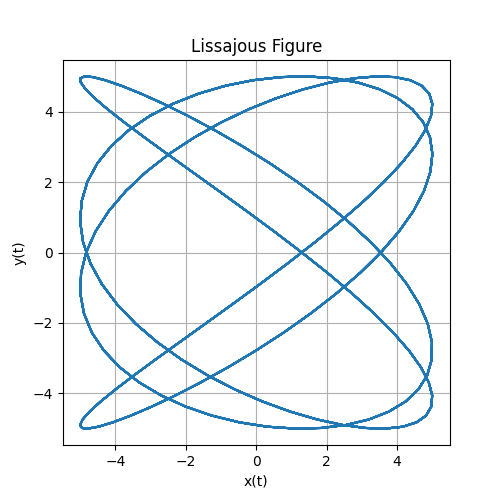
\includegraphics[width=0.5\textwidth]{figs/fig2_verify.png}
\end{figure}
\subsection{Case 3: $y = \sin(2\text{kHz} + 45^\circ)$, $x = \sin(3\text{kHz})$}

Given:
\[
x(t) = \sin(2\pi \cdot 3000 t)
\]
\[
y(t) = \sin(2\pi \cdot 2000 t + \frac{\pi}{4})
\]
\begin{align*}
x^2 + y^2 = \frac{1}{2} + \frac{1}{2} \sin\left( 4\pi \cdot 2000 t \right) + \sin^2\left( 2\pi \cdot 3000 t \right)
\end{align*}
The frequency ratio is:
\[
\frac{\omega_x}{\omega_y} = \frac{3000}{2000} = \frac{3}{2}
\]

The phase difference of \( 45^\circ \) will result in a skewed Lissajous figure with a diagonal symmetry.
\begin{figure}[H]
\centering
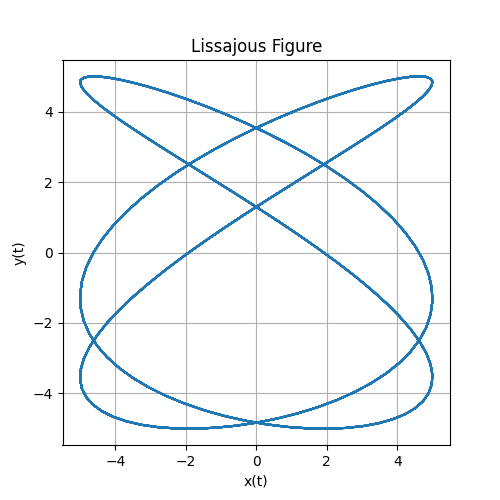
\includegraphics[width=0.5\textwidth]{figs/fig3.png}
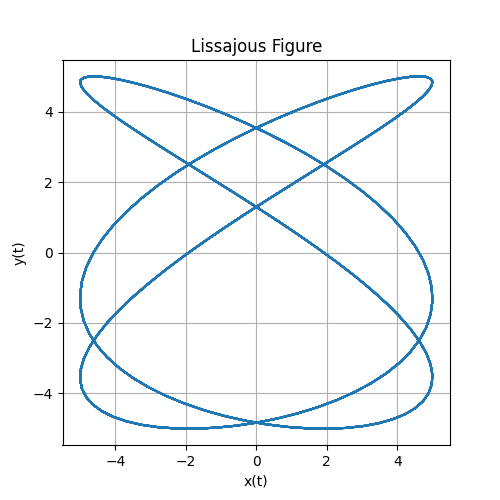
\includegraphics[width=0.5\textwidth]{figs/fig3_verify.png}
\end{figure}
\subsection{Case 4: $y = \sin(1\text{kHz})$, $x = \sin(3\text{kHz} + 45^\circ)$}

Given:
\[
x(t) = \sin(2\pi \cdot 3000 t + \frac{\pi}{4})
\]
\[
y(t) = \sin(2\pi \cdot 1000 t)
\]
\begin{align*}
x^2 + y^2 = \frac{1}{2} + \frac{1}{2} \sin\left( 4\pi \cdot 3000 t \right) + \sin^2\left( 2\pi \cdot 1000 t \right)
\end{align*}
The frequency ratio is:
\[
\frac{\omega_x}{\omega_y} = \frac{3000}{1000} = 3
\]

The phase difference of \( 45^\circ \) leads to a figure where the x-axis completes three cycles for every one cycle along the y-axis.
\begin{figure}[H]
\centering
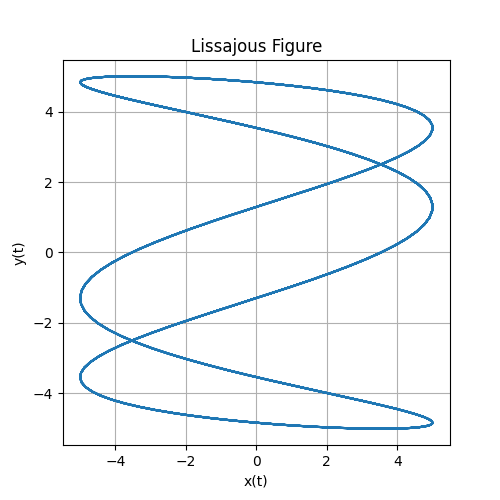
\includegraphics[width=0.5\textwidth]{figs/fig4.png}
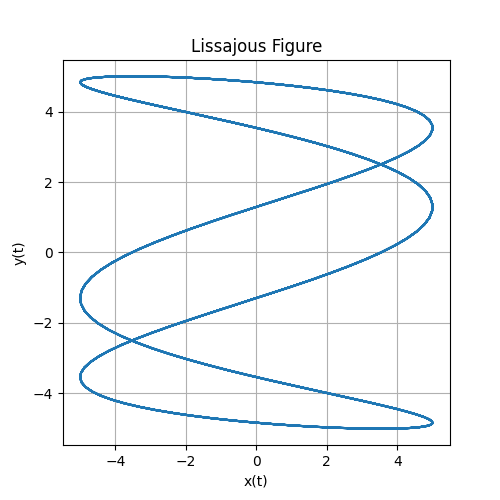
\includegraphics[width=0.5\textwidth]{figs/fig4_verify.png}
\end{figure}
\subsection{Case 5: $y = \sin(1\text{kHz})$, $x = \sin(2\text{kHz} + 45^\circ)$}

Given:
\[
x(t) = \sin(2\pi \cdot 2000 t + \frac{\pi}{4})
\]
\[
y(t) = \sin(2\pi \cdot 1000 t)
\]
\begin{align*}
x^2 + y^2 = \frac{1}{2} + \frac{1}{2} \sin\left( 4\pi \cdot 2000 t \right) + \sin^2\left( 2\pi \cdot 1000 t \right)
\end{align*}
The frequency ratio is:
\[
\frac{\omega_x}{\omega_y} = \frac{2000}{1000} = 2
\]

The phase difference of \( 45^\circ \) results in a Lissajous figure with two loops along the x-axis for every loop along the y-axis.
\begin{figure}[H]
\centering
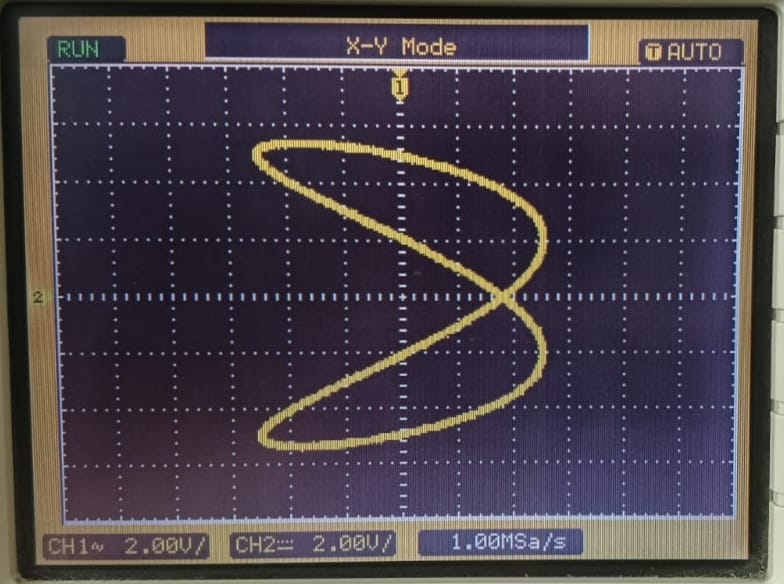
\includegraphics[width=0.5\textwidth]{figs/fig5.png}
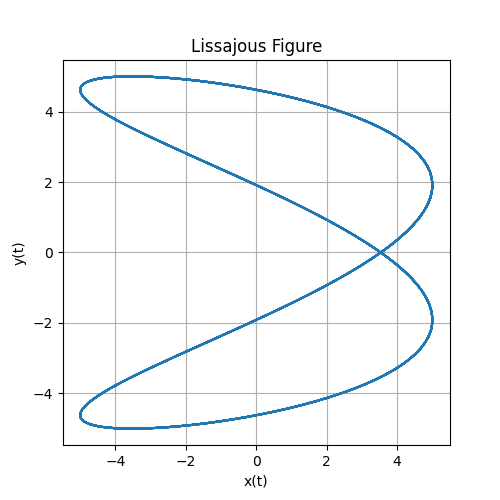
\includegraphics[width=0.5\textwidth]{figs/fig5_verify.png}
\end{figure}
\subsection{Case 6: $y = \sin(1\text{kHz})$, $x = \sin(1\text{kHz})$}

Given:
\[
x(t) = \sin(2\pi \cdot 1000 t)
\]
\[
y(t) = \sin(2\pi \cdot 1000 t)
\]
\begin{align*}
x = y
\end{align*}
The frequency ratio is:
\[
\frac{\omega_x}{\omega_y} = \frac{1000}{1000} = 1
\]

Since the frequencies are equal and there is no phase difference (\( 0^\circ \)), the resulting Lissajous figure is a straight line along the diagonal.
\begin{figure}[H]
\centering
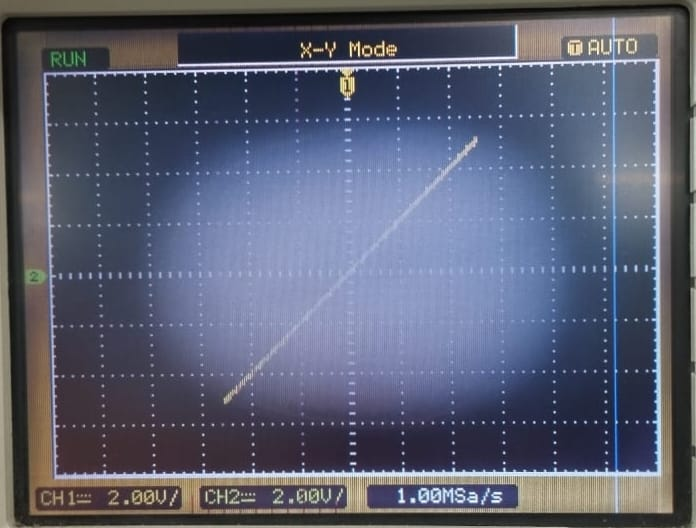
\includegraphics[width=0.5\textwidth]{figs/fig6.png}
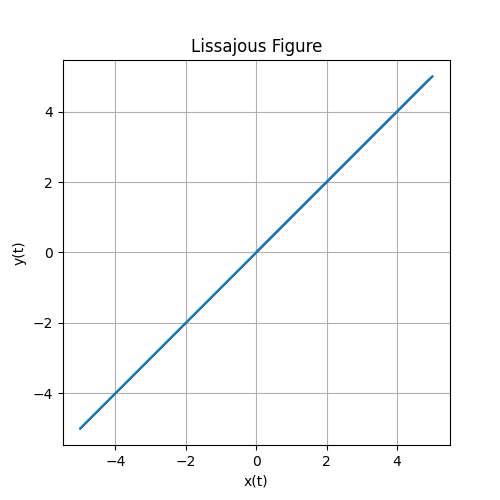
\includegraphics[width=0.5\textwidth]{figs/fig6_verify.png}
\end{figure}
\section{Voltage Range}
In all cases, the voltage variation is assumed to be in the range of $[-5, 5]V$.

\section{Conclusion}
Lissajous figures provide an elegant visualization of harmonic motion and phase relationships. Their study offers insights into signal analysis, mechanical vibrations, and artistic designs. Understanding their mathematical properties enhances their practical applications in science and engineering.\\
To capture a \textbf{one-time event} (also called a \textbf{single-shot event}) on a \textbf{Cathode Ray Oscilloscope (CRO)}, follow these steps:

\section{Digital Storage Oscilloscope (DSO),Cathode Ray Oscilloscope (CRO)}
\begin{figure}[H]
\centering
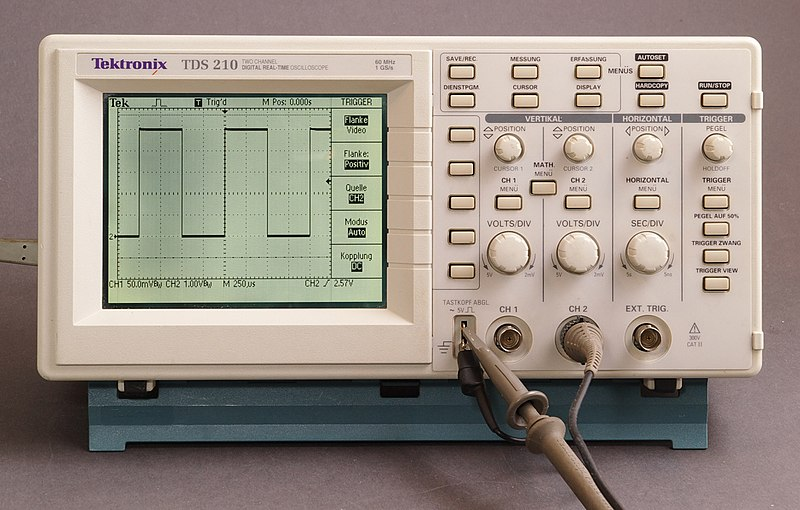
\includegraphics[width=0.5\textwidth]{figs/dso.png}
\caption{DSO}
\end{figure}

\begin{itemize}
    \item Traditional CROs do not have memory to store one-time events.
    \item A \textbf{DSO (Digital Storage Oscilloscope)} can capture and hold a transient signal.
\end{itemize}

\section{Adjust the Trigger Mode}
\begin{itemize}
    \item Set the \textbf{trigger mode} to \textbf{Single Shot} or \textbf{Single} (on DSOs).
    \item In a CRO, set the trigger to \textbf{Normal Mode} (not Auto) so it doesn't continuously refresh.
\end{itemize}

\section{Set the Trigger Level}
\begin{itemize}
    \item Adjust the \textbf{trigger level} to the expected signal amplitude.
    \item Choose a \textbf{trigger edge} (rising or falling) based on the signal behavior.
\end{itemize}

\section{Adjust Time Base and Voltage Scale}
\begin{itemize}
    \item Set the \textbf{time base} (horizontal scale) to match the expected event duration.
    \item Adjust the \textbf{voltage scale} (vertical sensitivity) for clear visibility.
\end{itemize}

\section{Capture the Event}
\begin{itemize}
    \item If using a CRO, once the event occurs, the screen will display it briefly.
    \item In a DSO, the captured waveform will be stored for later analysis.
\end{itemize}

\section{Freeze or Capture the Display}
\begin{itemize}
    \item A CRO cannot store waveforms, so you may need a \textbf{camera} to capture the screen.
    \item A DSO allows you to save and retrieve the waveform digitally.
\end{itemize}

\section{Alternative: Using a Storage Oscilloscope}
\begin{itemize}
    \item A \textbf{storage oscilloscope} can retain the waveform for a longer period using phosphor-based storage techniques.
\end{itemize}
Here is an image of a one time event captured on DSO of a sine wave produced by function generator:
\begin{figure}[H]
\centering
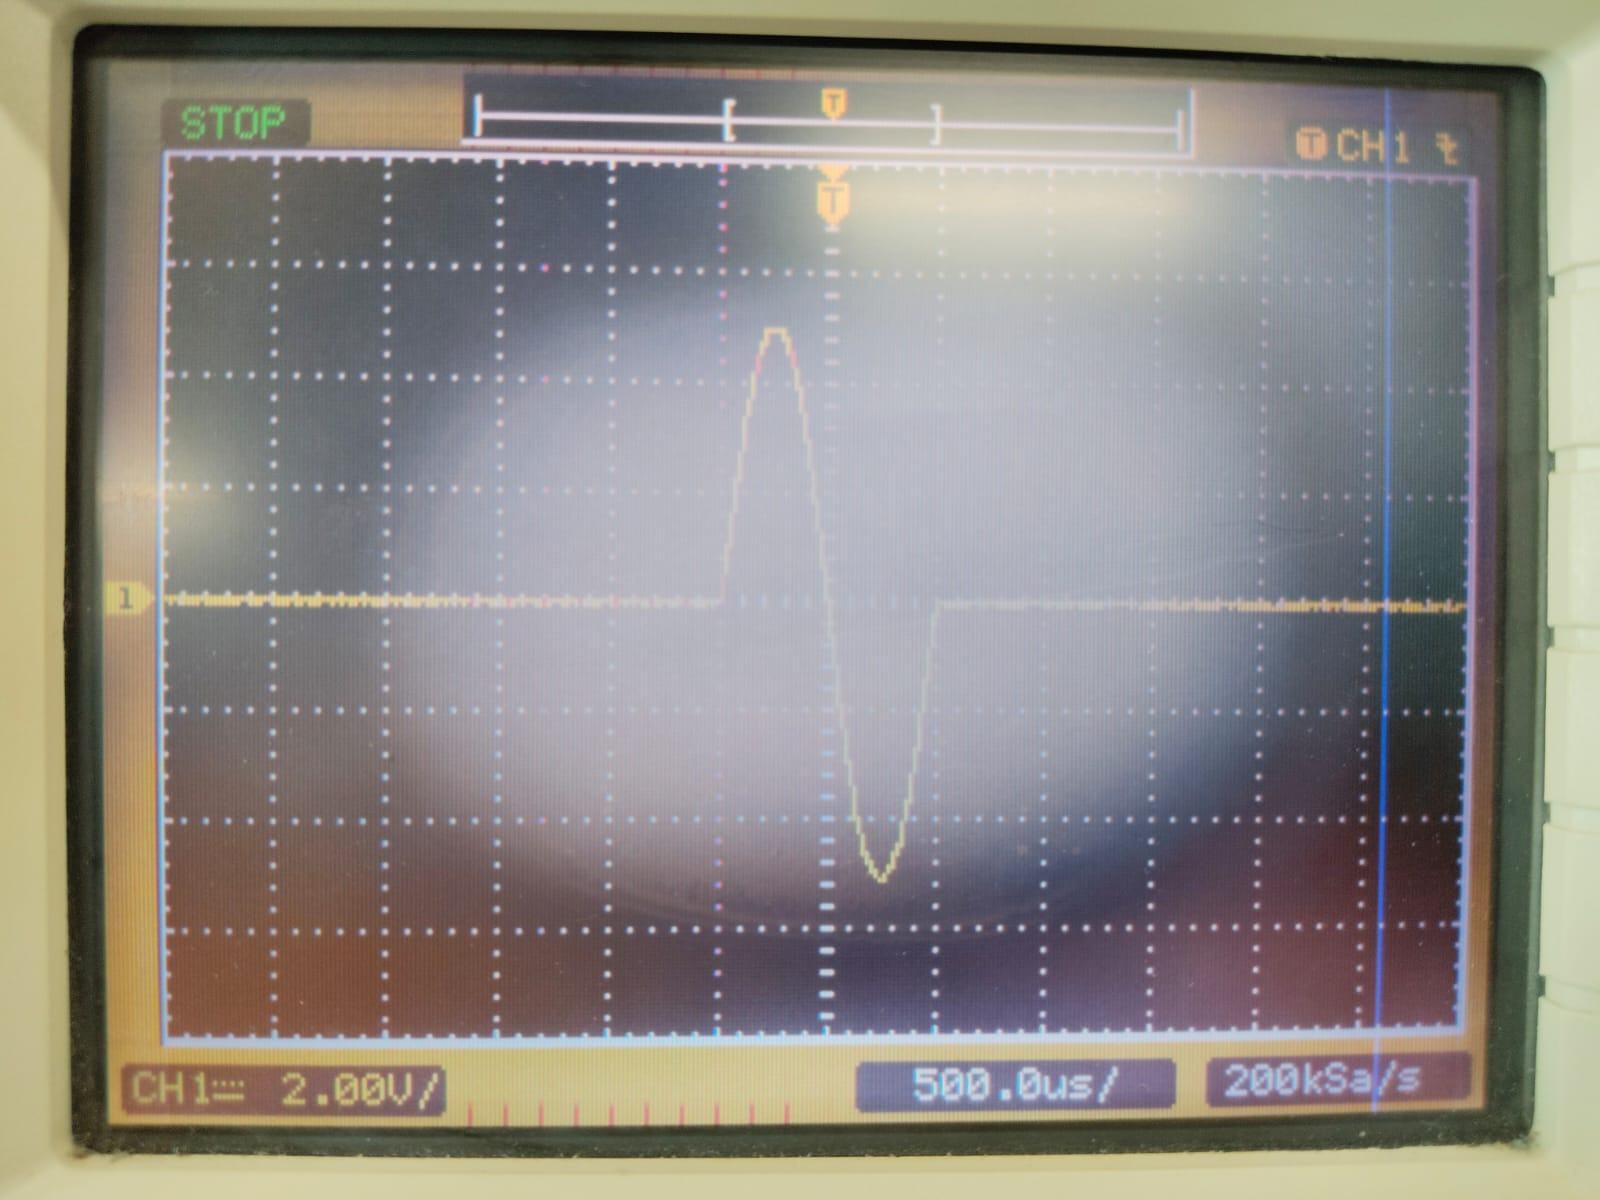
\includegraphics[width=0.6\textwidth]{figs/ofig1.png}
\end{figure}
Here is an image of a one time event captured on DSO of a square wave produced by function generator:
\begin{figure}[H]
\centering
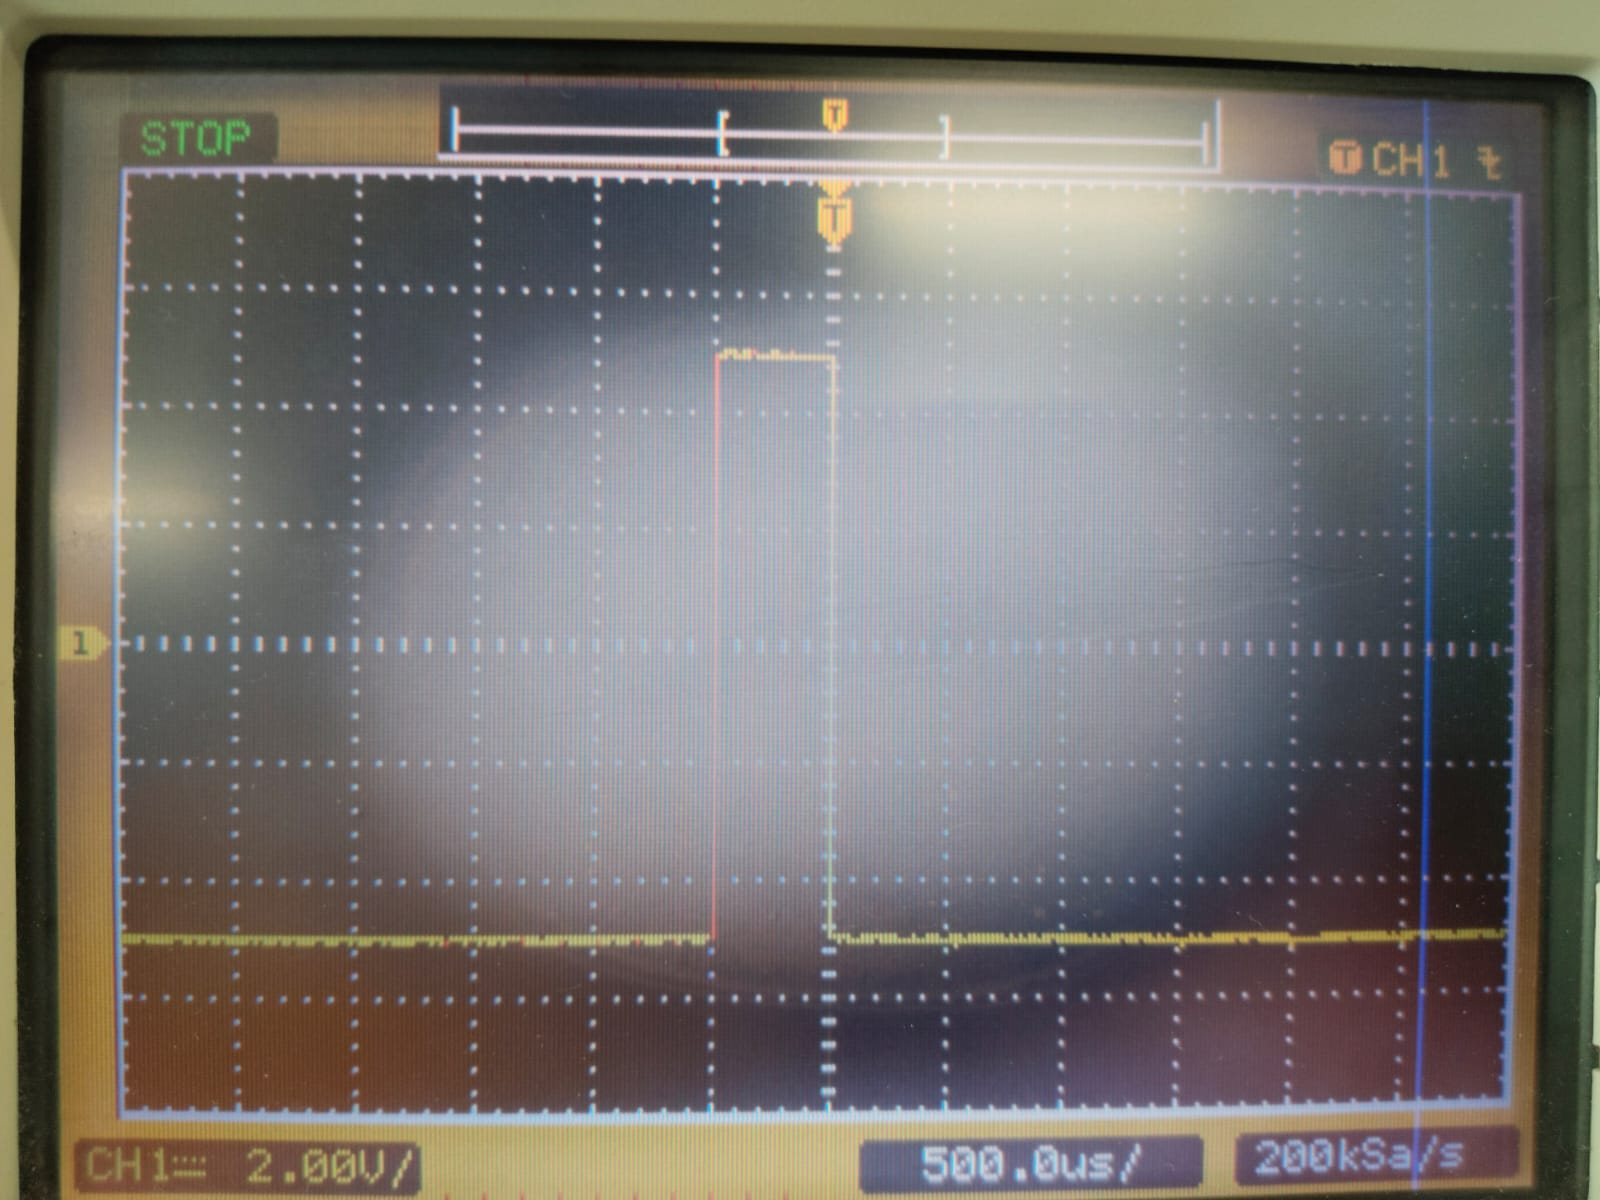
\includegraphics[width=0.6\textwidth]{figs/ofig2.png}
\end{figure}
\end{document}
